\chapter{Deployment}
\label{Deployment}
\section{Introduction}
In the following chapter, there is a walk-through on one of many ways to set up a secure pipeline. The pipeline starts with a source code, which will be explained further, and goes on with pushing the code to GitHub and further to \acrshort{aws}. Within these steps are the security measures and scans discussed previously. Some of these steps are automated using Terraform\footnote{Available at \url{https://www.terraform.io/}}, which is a \gls{infrastructure as code} tool. The group has found this repository to be a valuable resource \cite{aws-cicd-pipeline} and used Terraform AWS Documentation\footnote{Available at: \url{https://registry.terraform.io/providers/hashicorp/aws/latest}} for information on how to set up the different steps using Terraform. 
\\~\\
Below is a figure of the pipeline in \acrshort{aws}, showing its structure and how it is connected. The model is being built as the different steps in the pipeline are being presented.
\vspace{2mm}
\begin{figure}[H]
    \centering
    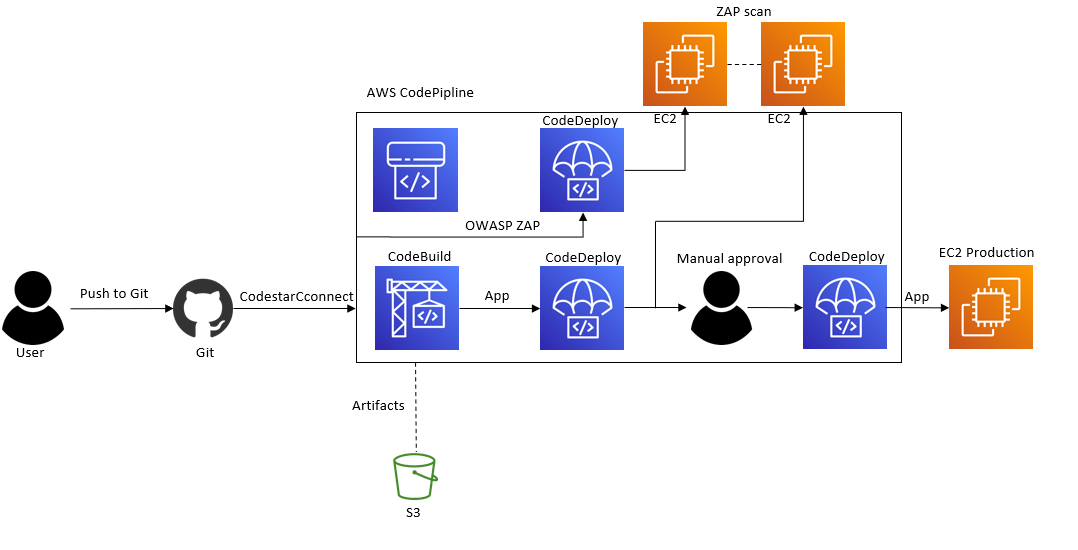
\includegraphics[width=1\columnwidth]{Images/aws-piplin-7.png}
    \caption{Pipline in AWS}
    \label{fig: Pipeline in AWS}
\end{figure}

\section{Code used in the pipeline}
For testing, the group decided on using OWASPs Juice Shop\footnote{Code available at \url{https://github.com/juice-shop/juice-shop}}, which is a deliberately vulnerable web application that is designed to help developers and others learn about web applications security concepts. The code is designed to simulate a real-world application by having common vulnerabilities within the code. The intention is to encourage users to find these vulnerabilities and exploit them and increase the understanding of web application security \cite{owaspJuiceShop}.
The code in the OWASP Juice Shop is open source code on GitHub and is written in TypeScript, which uses a Node.js server and Angular for \gls{front-end} \cite{owaspJuiceShopCode}.
The code contains different vulnerabilities, including \gls{SQL-injection}s, \gls{Cross-site scripting}, and many others. 
Overall, OWASP Juice Shop encourages users to improve their skills and it allows for customization and adaption for specific needs from the users. 

 
\section{Pushing to GitHub}
When the source code is ready to be pushed to GitHub, security measures must be in place. One of the previously mentioned measurements is branch protection. Branch protection rules are easy to enable in GitHub. It is done for each repository. GitHub has different branch protection rules one can enable, which are explained in \ref{branchprotection}. This can either be done in \gls{GUI} or automated using Terraform, which is shown in Appendix \ref{branchprotectionrules}. 
\\~\\
Further, the commit signature has to be configured. For signing commits in GitHub, one can either use an SSH or GPG key. These need to be generated and connected to the user's GitHub account.
GitHub provides documentation\footnote{Available at \url{https://docs.github.com/en/authentication/managing-commit-signature-verification/signing-commits}} on how to create a GPG and SSH keys, as well as how to connect these keys to a GitHub account.

\begin{figure}[H]
  \centering
  \begin{subfigure}[H]{0.4\textwidth}
    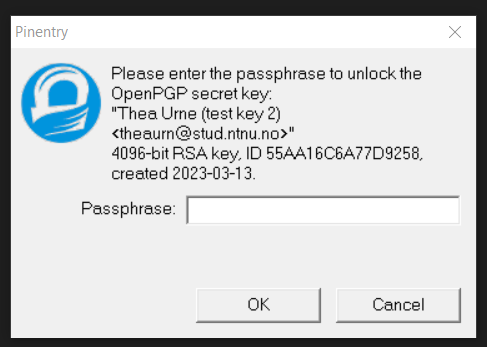
\includegraphics[width=\textwidth]{Images/signedcommits.png}
    \caption{Required passphrase when committing to GitHub}
    \label{fig:image1}
  \end{subfigure}
  \hfill
  \begin{subfigure}[H]{0.4\textwidth}
    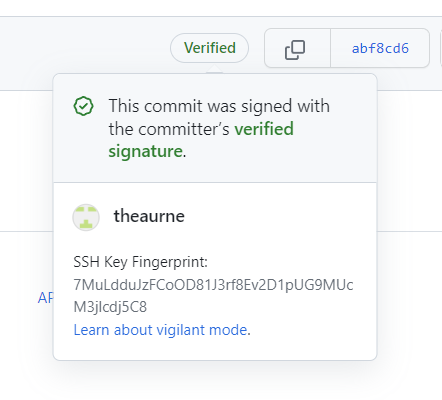
\includegraphics[width=\textwidth]{Images/verified-commit.png}
    \caption{Verified commit}
    \label{fig:image2}
  \end{subfigure}
  \caption{Required signed commits}
  \label{fig:overall}
\end{figure}

\vspace{2mm}
\begin{figure}[H]
    \centering
    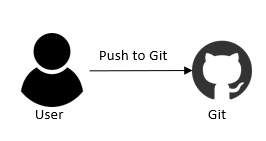
\includegraphics[width=0.5\columnwidth]{Images/aws-piplin-1.png}
    \caption{Pushing the source code to GitHub}
    \label{fig: Pushing the source code to GitHub}
\end{figure}


\section{Managing security in GitHub}
When the source code is securely pushed to its belonging branch and is being merged into the main branch, CodeQL needs to scan the code for vulnerabilities. This is done by setting up CodeQL\footnote{Instructions available at \url{https://docs.github.com/en/code-security/code-scanning/automatically-scanning-your-code-for-vulnerabilities-and-errors/configuring-code-scanning-for-a-repository}} and customizing the trigger for the code scan. 
\\~\\
Setting up CodeQL is done by adding the CodeQL YAML file to the workflow, which contains the configuration settings for running the analysis. To customize the trigger for the analysis, the pull request and push events are added to the workflow file, causing the analysis to run automatically whenever a pull request or push is made to the specified branch. The branch specified in this case is the main branch. \cite{CodeQLCustom}

\begin{tcolorbox}
\begin{verbatim}
on:
  push:
    branches: [main]
  pull_request:
    branches: [main]
\end{verbatim}
\end{tcolorbox}

 Other security tools in GitHub are Dependabot\footnote{Instructions available at \url{https://docs.github.com/en/code-security/dependabot/dependabot-security-updates/configuring-dependabot-security-updates}} and Secret scanner\footnote{Instructions available at \url{https://docs.github.com/en/code-security/secret-scanning/configuring-secret-scanning-for-your-repositories}}. These are also enabled in the security settings. After being enabled, all these tools automatically scan the code for vulnerabilities.

\begin{figure}[H]
    \centering
    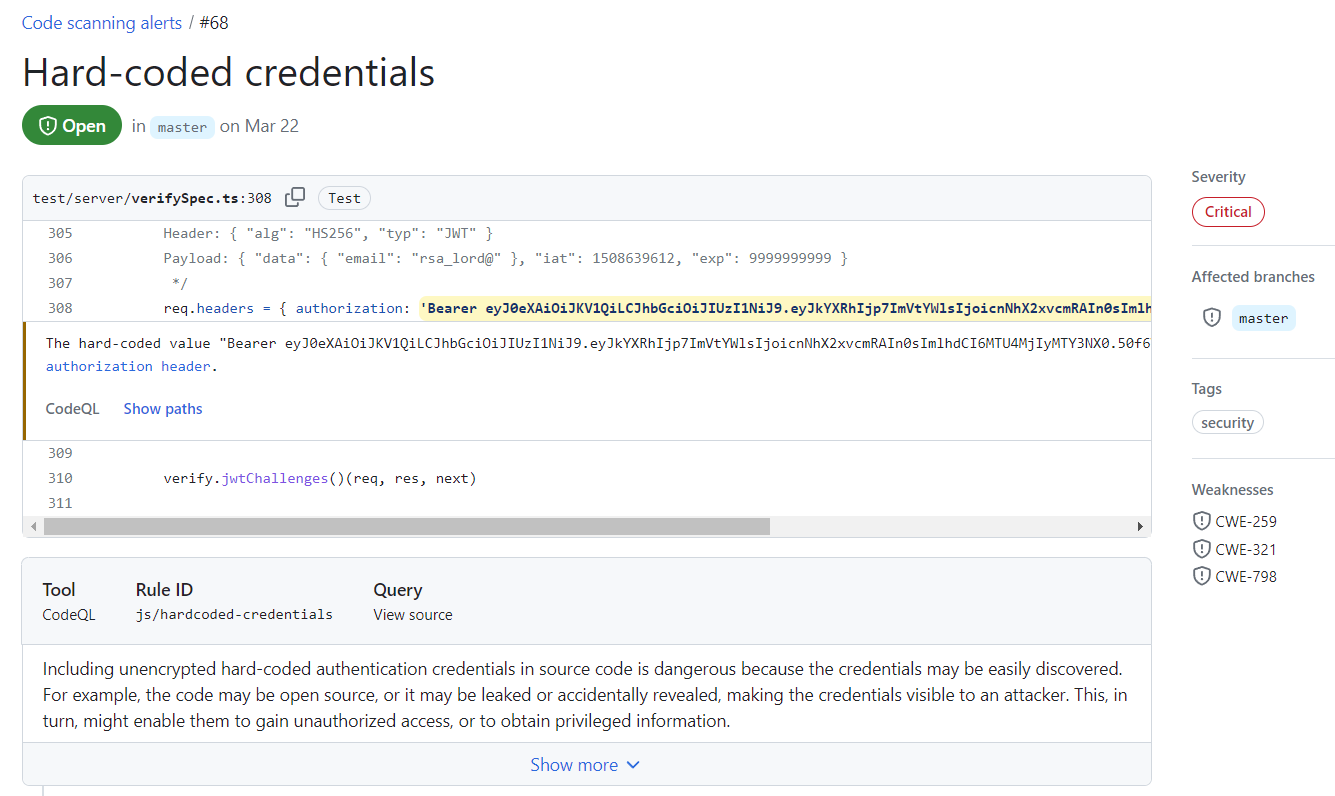
\includegraphics[width=0.8\columnwidth]{Images/codescan.png}
    \caption{Critical alert from CodeQL}
    \label{fig: Critical alert CodeQL}
\end{figure}

An example of code scanning alerts using CodeQL is this critical alert, notifying the user of a hard-coded credential. This alert is shown in a pull request from a branch to the main branch. The code scanning alerts refer to CWE weaknesses, which are explained further in \ref{cwe}.

\vspace{2mm}
\begin{figure}[H]
    \centering
    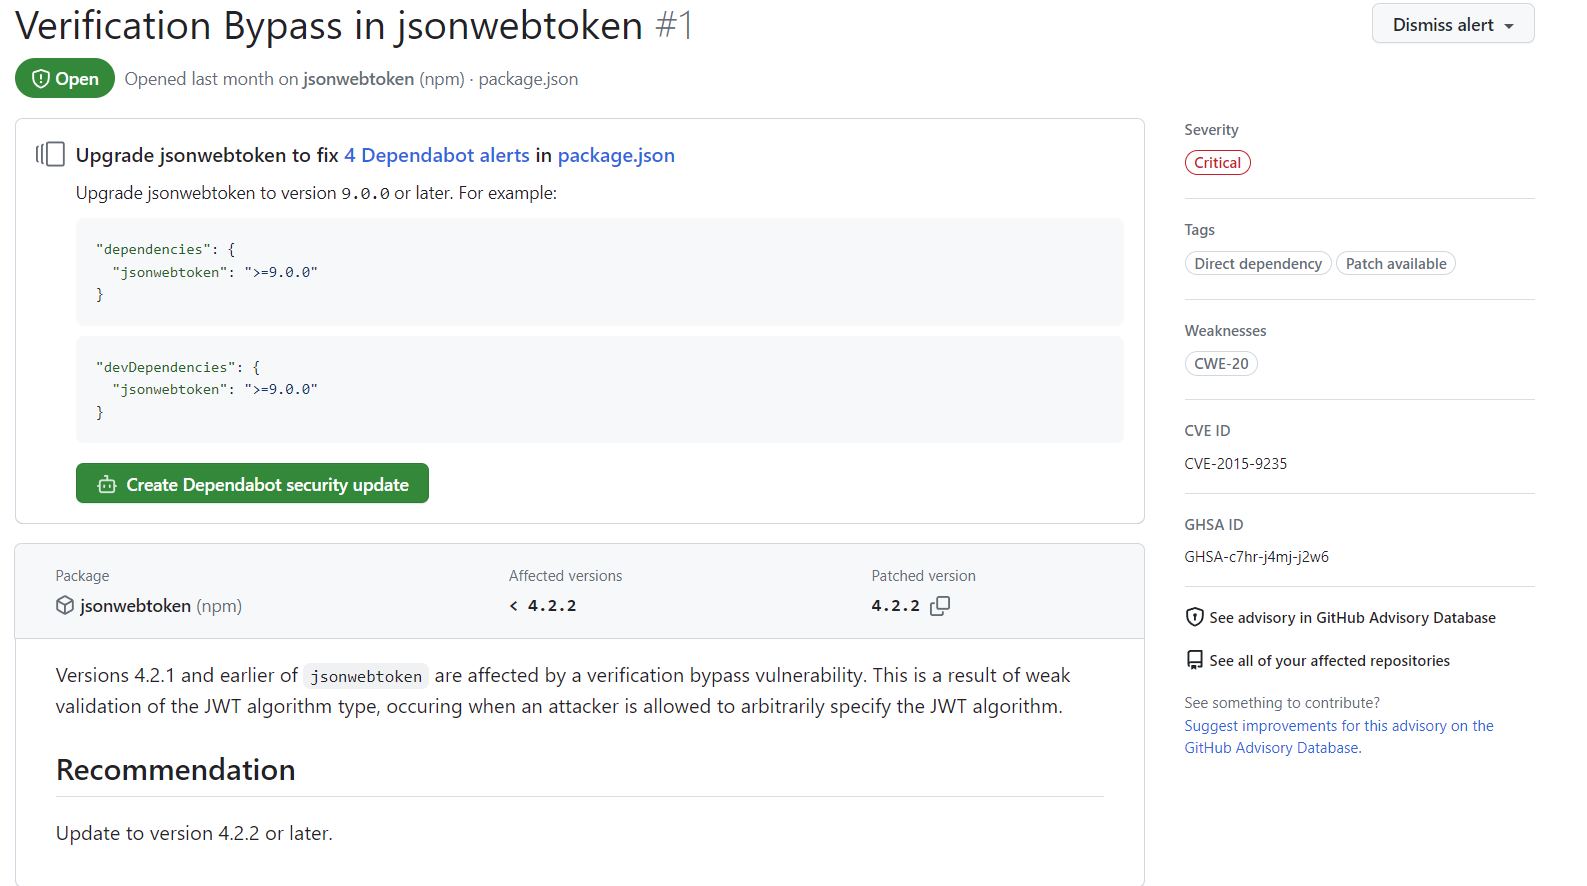
\includegraphics[width=0.8\columnwidth]{Images/dependabotalert.png}
    \caption{Critical alert from Dependabot}
    \label{fig: Critical alert from Dependabot}
\end{figure}

Figure \ref{fig: Critical alert from Dependabot} is one of the critical alerts from Dependabot in the Juice-Shop repository. It shows a vulnerability in the dependency version used, following a suggestion on a patched version. Dependabot, similarly to CodeQL, refers to CWE weaknesses. Additionally, it refers to a CVE ID. 

\vspace{2mm}
\begin{figure}[H]
    \centering
    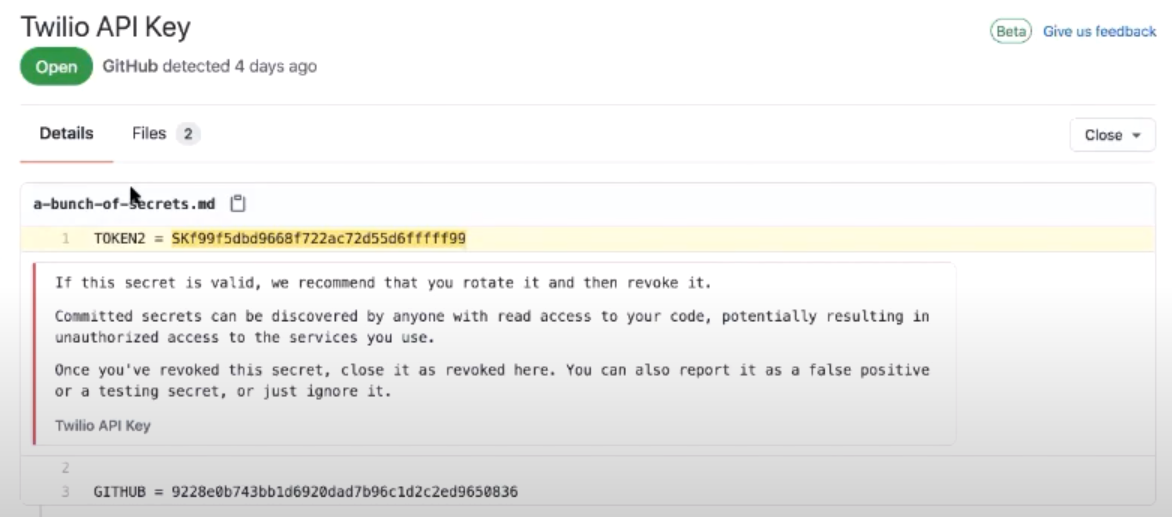
\includegraphics[width=0.8\columnwidth]{Images/secretscanneralert.png}
    \caption{Alert from secret scanner} Adapted from: \cite{GitHubVideo}
    \label{fig: Alert from secret scanner}
\end{figure}
The GitHub Secret scanner did not detect any secrets in the Juice-Shop repository. Therefore, Figure \ref{fig: Alert from secret scanner} is taken from GitHub's demonstration of the secret scanner \cite{GitHubVideo}. The alert warns the user about an API key that matches the pattern of their partner Twilio. 

\section{Committing the source code to AWS}
When the source code is pushed to the main branch in the GitHub repository, the source code can be built in \acrshort{aws}. In order for this to be done, a connection between the \acrshort{aws} and GitHub account needs to be made. This can be done using \acrshort{aws} CodeStar Connections\footnote{A tool that enables CodePipeline to connect to third-party repositories \cite{CodeStarConnections}.}. By creating this connection as a resource, it can be used by \acrshort{aws} CodePipeline to automatically trigger the pipeline in response to any changes made to the GitHub repository.
This can either be done on the \acrshort{aws} website or by using Terraform to create a connection resource with GitHub as the provider.

\begin{tcolorbox}
\begin{verbatim}
resource "aws_codestarconnections_connection" "code-connection" {
  name          = "code-connection"
  provider_type = "GitHub"
}    
\end{verbatim}
\end{tcolorbox}

After successfully creating the connection resource in \acrshort{aws} with Terraform, it is necessary to perform a manual verification process in \acrshort{aws}. This step is crucial because it is not possible to pass secrets through \acrshort{aws} to GitHub login, as the connection opens a third-party login page that \acrshort{aws} does not control. Therefore, it is essential to log in to the system with one's GitHub account credentials.

\vspace{2mm}
\begin{figure}[H]
    \centering
    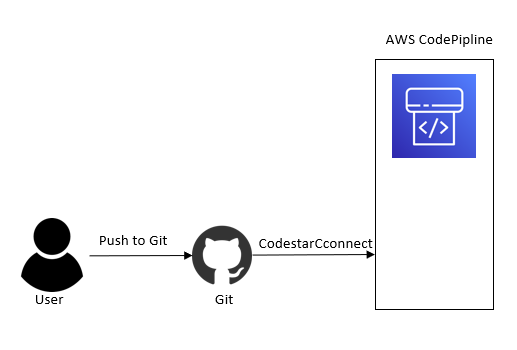
\includegraphics[width=0.6\columnwidth]{Images/aws-piplin-2-1.png}
    \caption{Committing the source code to AWS}
    \label{fig: Committing the source code to AWS}
\end{figure}

\section{Storing artifacts}
To store \gls{artifact}s generated during different stages of the pipeline, an S3 bucket is created. The bucket is created as a resource with optional variables. One crucial aspect to consider is the need for unique bucket names within the server area, as \acrshort{aws} uses this as a means to differentiate between buckets owned by different users. Either the name can be configured like in the code below, or the name variable can be excluded and \acrshort{aws} will configure the name themselves.

\begin{tcolorbox}
\begin{verbatim}
resource "aws_s3_bucket" "codepipeline_artifact" {
  bucket = "artifact-bucket-unique-name"
}
\end{verbatim}
\end{tcolorbox}

For each stage to be able to access the S3 bucket and retrieve the last stage's \gls{artifact}s, it has to be given access to the bucket. These access rights have to be individually given to each stage in the pipeline. In the following code the pipeline and every stage are given access to the bucket, hence the "s3:*".

\begin{tcolorbox}
\begin{verbatim}
statement {
    sid       = ""
    actions   = ["s3:*", "codebuild:*"]
    resources = ["*"]
    effect    = "Allow"
}
\end{verbatim}
\end{tcolorbox}

\vspace{2mm}
\begin{figure}[H]
    \centering
    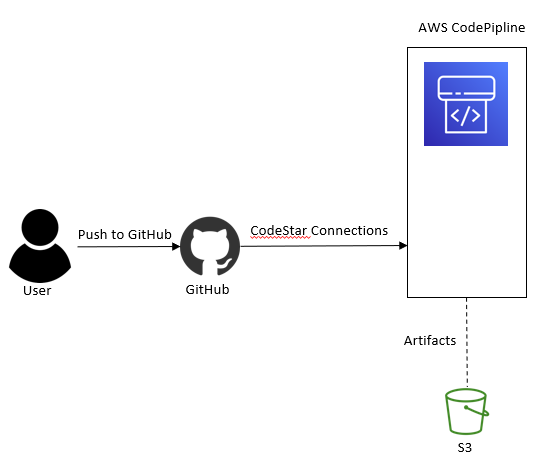
\includegraphics[width=0.6\columnwidth]{Images/aws-piplin-2.png}
    \caption{Storing the artifacts in an S3 Bucket}
    \label{fig: Storing the artifacts in an S3 Bucket}
\end{figure}

\section{Build stage}
In the build stage, CodePipeline uses CodeBuild to compile the source code into a working website. CodeBuild uses a \say{build project} that is created using the code in Appendix X. This build project is used to create the \say{build environment}, which is what operating system, Docker image, and compute- resources and types are used.  It is possible to choose from various compute- environments and types\footnote{Available at \url{https://docs.aws.amazon.com/codebuild/latest/userguide/build-env-ref-compute-types.html}}. In this example, the environment type is set to be a Linux container. The compute type refers to the amount of memory, CPUs, and disk space needed, which in this case is set to be the smallest amount. 

\begin{tcolorbox}
\begin{verbatim}
environment {
    compute_type                = "BUILD_GENERAL1_SMALL"
    image                       = "aws/codebuild/standard:6.0"
    type                        = "LINUX_CONTAINER"
    image_pull_credentials_type = "CODEBUILD"
  }
\end{verbatim}
\end{tcolorbox}

Further, the build project downloads the source code and uses build commands, found in the \gls{buildspec} file, to run the build. The source code is retrieved from the S3 bucket, where it was put from the previous stage. \cite{CodeBuildProcess}
dette er et 
\vspace{2mm}
\begin{figure}[H]
    \centering
    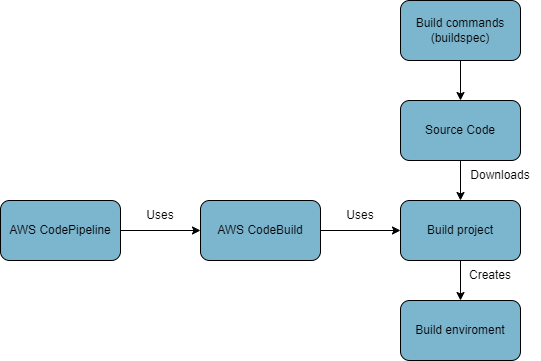
\includegraphics[scale=0.4]{Images/CodeBuild.drawio.png}
    \caption{AWS CodeBuild} 
    \label{fig: AWS CodeBuild}
\end{figure}

\vspace{2mm}
\begin{figure}[H]
    \centering
    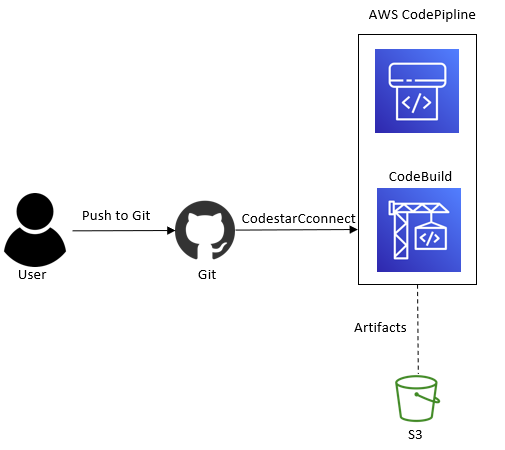
\includegraphics[width=0.6\columnwidth]{Images/aws-piplin-3.png}
    \caption{CodePipeline using CodeBuild}
    \label{fig: CodePipeline using CodeBuild}
\end{figure}

\section{Deployment to testing}
\label{Deployment to testing}
\subsection{Setting up for CodeDeploy}
In the deployment stage, an application refers to the combination of deployment groups and deployments that keep track of all the necessary components. The deployment group specifies the configurations to use for the deployment and also specifies which preconfigured instance\footnote{Available at \url{https://docs.aws.amazon.com/AWSEC2/latest/UserGuide/EC2_GetStarted.html}} to use for the deployment. The deployment itself deploys the given revision, which typically consists of the source code for an application. In addition, an \gls{appspec} file is added to the revision. 

\vspace{2mm}
\begin{figure}[H]
    \centering
    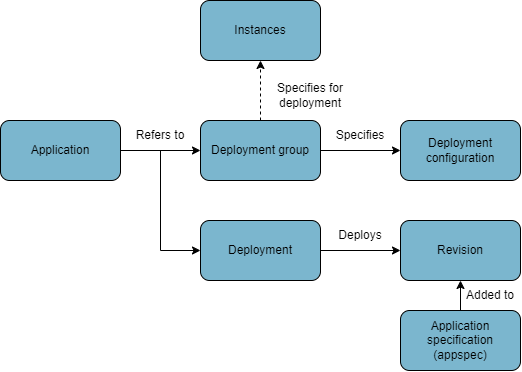
\includegraphics[width=0.6\columnwidth]{Images/CodeDeploy.drawio.png}
    \caption{AWS CodeDeploy using two \acrshort{ec2} instances}
    \label{fig: AWS CodeDeploy using two EC2 instances}
\end{figure}
\newpage

\subsection{Setting up for testing}

This stage utilizes two \acrshort{ec2} instances: one for OWASP Zap and the other for the application. The reason for setting up two instances separately is to make it easier to manage each program by separating them. This setup also allows for easier reuse of code when deploying the application into production, as well as easier integration of both instances with other programs or changes. However, both instances utilize the same S3 bucket, but the files are separated into two different directories so they do not interfere with each other.

\vspace{2mm}
\begin{figure}[H]
    \centering
    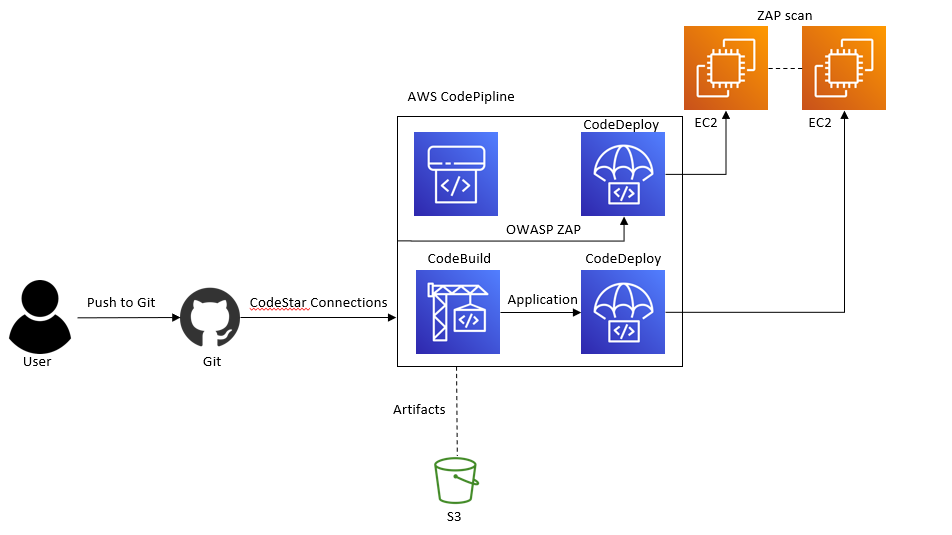
\includegraphics[width=0.6\columnwidth]{Images/aws-piplin-5.png}
    \caption{Deployment to testing}
    \label{fig: Deployment to testing}
\end{figure}

For OWASP Zap to be able to scan the application, the instances need to communicate. To enable communication between the \acrshort{ec2} instances within the \acrlong{vpc}, individual network interfaces have been allocated to each instance with a single IP address. This method guarantees that both instances can always find each other because the IP address will always be the same for both instances.

\begin{tcolorbox}
\begin{verbatim}
resource "aws_network_interface" "interface_network1" {
  subnet_id   = aws_subnet.my_subnet.id
  private_ips = ["172.16.10.100"]
}

resource "aws_network_interface" "interface_network2" {
  subnet_id   = aws_subnet.my_subnet.id
  private_ips = ["172.16.10.101"]
}
\end{verbatim}
\end{tcolorbox}

The security tests are conducted by setting up a docker container\footnote{Available at \url{https://www.docker.com/resources/what-container/}} on the \acrshort{ec2} instance created for OWASP Zap, which runs one of the automated standard tests predefined by OWASP ZAP. The container uses the \say{weekly stable image} of OWASP Zap\footnote{Available at \url{https://www.zaproxy.org/docs/docker/}}. Although these tests are typically customized to suit the specific requirements of an application, for this demo, the predefined tests are satisfactory. Once the container is launched, the scan is directed towards the other instance in the \acrshort{vpc}, and the output obtained resembles the following.

\vspace{2mm}
\begin{figure}[H]
    \centering
    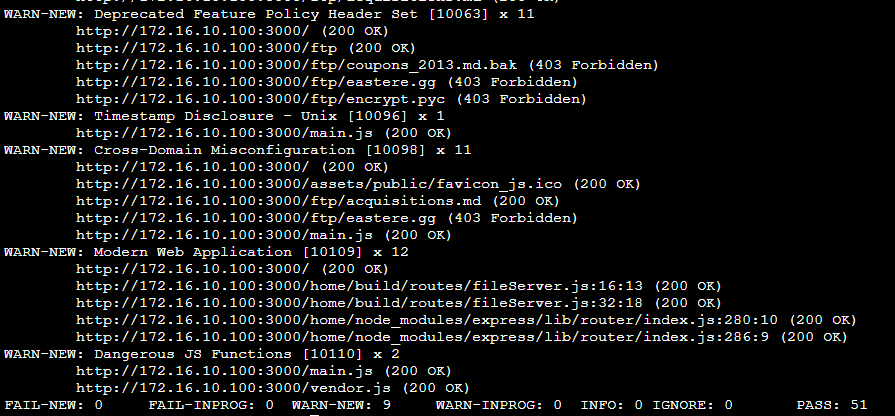
\includegraphics[width=0.8\columnwidth]{Images/owasp-zap-scan.png}
    \caption{OWASP Zap baseline scan}
    \label{fig: OWASP Zap baseline scan}
\end{figure}


\section{Deployment to production}
In the production stage, CodePipeline utilizes CodeDeploy, as described in \ref{Deployment to testing}. Before the code gets moved to production, it needs to be accepted by manual approval by a user in \acrshort{aws}. The purpose of this step is to allow for a review of the results from the automated security tests, to
ensure that no faulty code is deployed. When new code or changes have gone through testing, a notification will occur in the \acrshort{sns} topic\footnote{\acrshort{sns} is a service that provides message delivery to a topic. A topic is the communication channel the users can subscribe to \cite{SNStopic}.} created. Someone then has to manually accept the code waiting to be moved to production.

\vspace{2mm}
\begin{figure}[H]
    \centering
    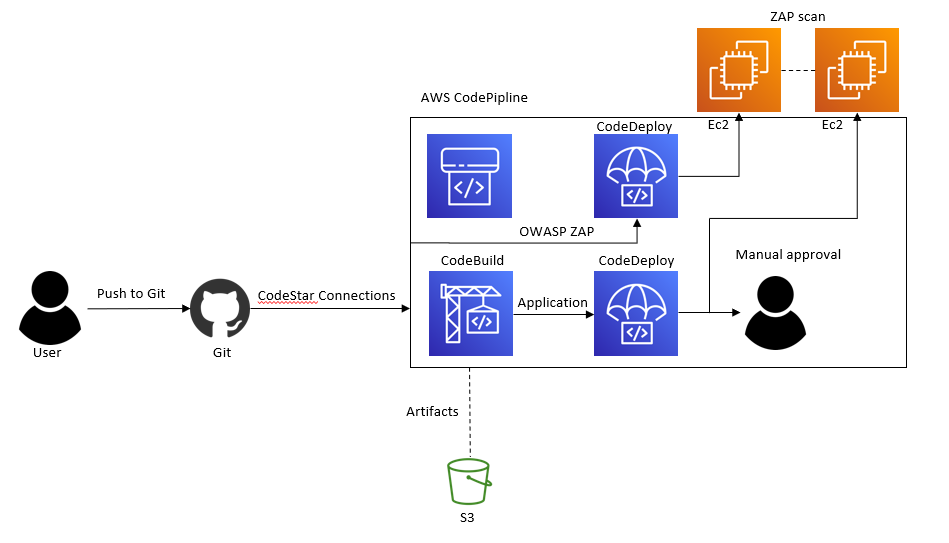
\includegraphics[width=0.8\columnwidth]{Images/aws-piplin-6.png}
    \caption{Manual approval before deploying the application}
    \label{fig: Manual approval before deploying the application}
\end{figure}

After the manual approval process is completed, the code will be deployed to production in a similar manner to the process described in \ref{Deployment to testing}. After all these steps are complete, the pipeline results in the pipeline displayed in Figure \ref{fig: Finished pipeline created in AWS}.\footnote{Complete code available at \url{https://github.com/DCSG2900-Bachelor-thesis/CodePipeline}}

\vspace{2mm}
\begin{figure}[H]
    \centering
    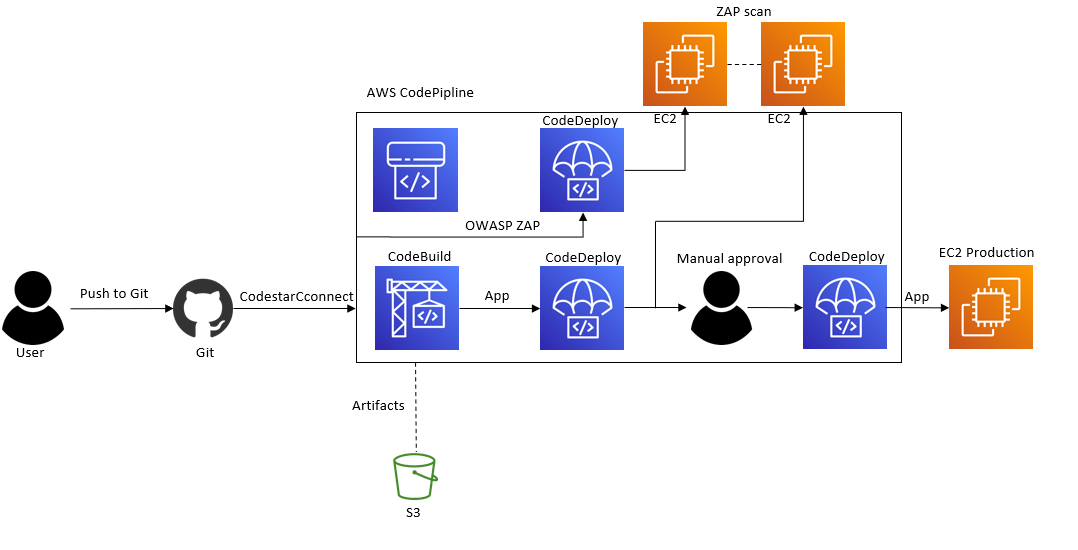
\includegraphics[width=0.8\columnwidth]{Images/aws-piplin-7.png}
    \caption{Finished pipeline created in \acrshort{aws}}
    \label{fig: Finished pipeline created in AWS}
\end{figure}